\documentclass[12pt]{standalone}
\usepackage{amsmath}
\usepackage{pgfplots}
\pgfplotsset{compat=1.15}
\usepgfplotslibrary{fillbetween}

\begin{document}
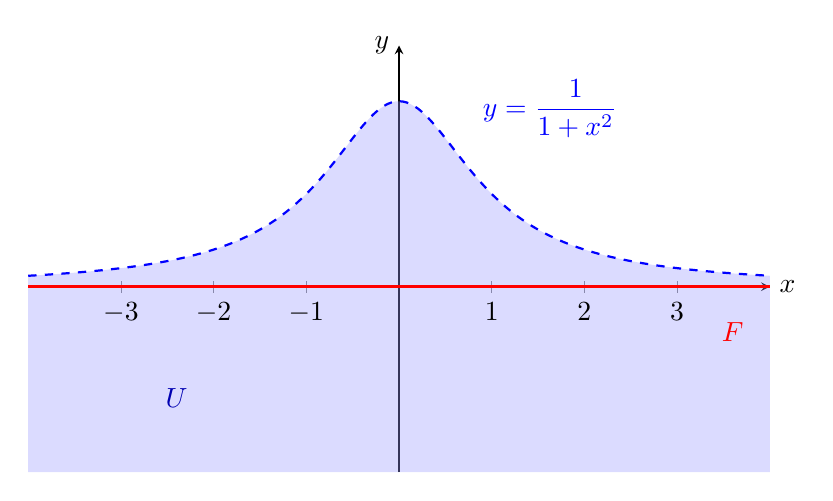
\begin{tikzpicture}
\begin{axis}[
    axis lines=middle,
    xmin=-4, xmax=4,
    ymin=-1, ymax=1.3,
    xlabel={$x$}, ylabel={$y$},
    xlabel style={at={(ticklabel* cs:1)}, anchor=west},
    ylabel style={at={(ticklabel* cs:1)}, anchor=east},
    xtick={-3,-2,-1,1,2,3},
    ytick=\empty, % {-1,1},
    width=11cm, height=7cm,
    clip=true,
]
% region U: everything strictly below the curve
\addplot[name path=curve, draw=none, domain=-4:4, samples=100] {1/(1+x^2)};
\addplot[name path=bottom, draw=none] coordinates {(-4,-1) (4,-1)};
\addplot[blue!40, fill opacity=0.35] fill between[of=curve and bottom];

% boundary of U (not contained in U): dashed
\addplot[blue, dashed, thick, domain=-4:4, samples=100, smooth] {1/(1+x^2)};
\node[blue, anchor=south west] at (axis cs:0.8,0.75) {$y=\dfrac{1}{1+x^2}$};

% F: the x-axis
\addplot[red, very thick, domain=-4:4] {0};

\node[blue!70!black] at (axis cs:-2.4,-0.6) {$U$};
\node[red, anchor=south] at (axis cs:3.6,-0.35) {$F$};
\end{axis}
\end{tikzpicture}
\end{document}
